\documentclass[border=0.2cm]{standalone}
\usepackage{tikz}
\usetikzlibrary{intersections,calc}
\begin{document}


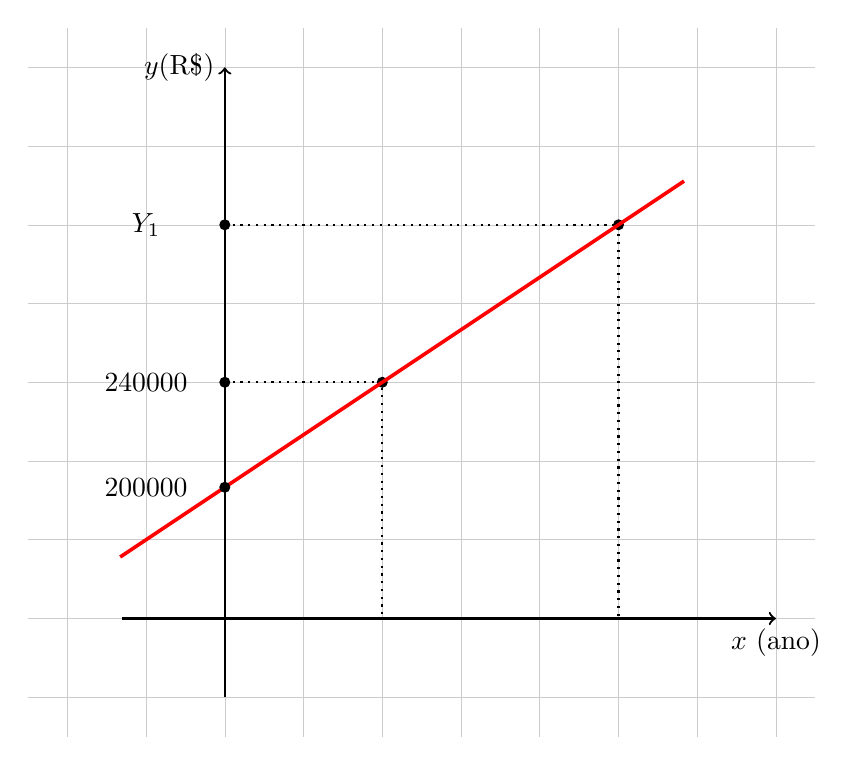
\begin{tikzpicture}
  \coordinate (a) at (0,0); 
  \coordinate (b) at (2,3);
  \coordinate (bx) at (0,3);
  \coordinate (by) at (2,0);
  \coordinate (c) at (5,5);
  \coordinate (cx) at (0,5);
  \coordinate (cy) at (5,0);
 

  \draw[help lines,black!20] (-2.5,-1.5) grid (7.5,7.5);
  %\foreach \x in {1,...,6} \node[left] at (0,\x) {\x} node[below] at (\x,0) {\x};
  \draw[thick,->,name path=yline] (0,-1) -- (0,7)   node[left]   {$y$(R\$)};
  \draw[thick,->] (-1.3,0) -- (7,0) node[below] {$x$ (ano)};
  \draw[thick, dotted] (cx) -- (c) -- (cy);
  \draw[thick, dotted] (bx) -- (b) -- (by);
  \fill[color=black] (b) circle (2pt);% node[right] {(b)};
  \fill[color=black] (c) circle (2pt);% node[right] {(c)};
  \fill (bx) circle (2pt) node[xshift=-1cm] {$240000$};
  \fill (cx) circle (2pt) node[xshift=-1cm] {$Y_1$};

  \draw[line width=1.3pt,red,name path=redline] ($(b)!-4cm!(c)$) -- ($(c)!-1cm!(b)$);
  \fill [name intersections={of=yline and redline}] (intersection-1) circle (2pt) 
      node[xshift=-1cm] {$200000$};
  

  %\draw (-2,0) circle (1pt) node[left] {$f(x_1)$};
  %\draw (-2,1) circle (1pt) node[left] {$f(x_2)$};
%  %\draw[thick, dotted] (-2,1) -- +(3,0) -- (1,-1) node[below] {$x_2$};
%  %\draw[thick, dotted] (0,0) -- (1,0);
%  %\draw[thick] (.5,0) arc (0:45:0.5) node[right] {$\alpha$};
%  %\fill (1,1) circle (1.2pt);
%  %\fill (0,0) circle (1.2pt);
\end{tikzpicture}



\end{document}